%%%%%%%%%%%%%%%%%%%%%%%%%%%%%%%%%%%%%%%%%%%%%%%%%%%%%%%%%%%%%%%%%%%%%%%%%%
%%%%%                        Intro Générale                         %%%%%%
%%%%%%%%%%%%%%%%%%%%%%%%%%%%%%%%%%%%%%%%%%%%%%%%%%%%%%%%%%%%%%%%%%%%%%%%%%
\phantomsection 
\addcontentsline{toc}{chapter}{General introduction}
\addtocontents{toc}{\protect\addvspace{10pt}}

\vspace*{-1cm}
\begin{flushright}
\section*{\fontsize{20pt}{20pt}\selectfont\textnormal{General introduction}}
\end{flushright}
\vspace{2cm}

\lhead[\fancyplain{}{General introduction}]
      {\fancyplain{}{}}
\chead[\fancyplain{}{}]
      {\fancyplain{}{}}
\rhead[\fancyplain{}{}]
      {\fancyplain{}{General introduction}}
\lfoot[\fancyplain{}{}]%
      {\fancyplain{}{}}
\cfoot[\fancyplain{}{\thepage}]
      {\fancyplain{}{\thepage}}
\rfoot[\fancyplain{}{}]%
     {\fancyplain{}{\scriptsize}}
     

%%%%%%%%%%%%%%%%%%%%%%%%%%%%%%%%%%%%%%%%%%%%%%%%%%%%%%%%%%%%%%%%%%%%%%%%%%
%%%%%                      Start part here                          %%%%%%
%%%%%%%%%%%%%%%%%%%%%%%%%%%%%%%%%%%%%%%%%%%%%%%%%%%%%%%%%%%%%%%%%%%%%%%%%%

This doctoral thesis has been undertaken from December 2nd, 2019 to November 30th, 2022, at the LJK (Laboratoire Jean Kuntzmann for applied mathematics and informatics) in Grenoble, France. It was funded by the French National Center for Scientific Research, as the result of a collaboration between the PPrime Institute (UPR3346, Poitiers, France), the French Cycling Federation (FFC), and the INSEP (French National Institute of Sport, Expertise and Performance), through the CREPS of Poitiers (Center for Sport Resource, Expertise, and Performance) and TSF Voiron (Springboard for Sports Training). It was later incorporated within the Perf'Analytics framework, which aims to boost French sports performance towards the 2024 Olympic Games in Paris, with a particular focus on video analysis.

\vspace*{0.5cm}

This work led to the publication of 3 peer-reviewed articles, 1 conference paper, and the release of an open-source package. Another peer-reviewed article has been published during this period, although it is not related to the program \cite{Pagnon2022d}.

\noindent\cite{Pagnon2021}: David Pagnon, Mathieu Domalain and Lionel Reveret. \textit{Pose2Sim: An
End-to-End Workflow for 3D Markerless Sports Kinematics—Part 1:
Robustness.} Sensors, vol. 21, no. 19, 2021.

\noindent\cite{Pagnon2022a}: David Pagnon, Mathieu Domalain and Lionel Reveret. \textit{Pose2Sim: An
End-to-End Workflow for 3D Markerless Sports Kinematics—Part 2:
Accuracy.} Sensors, vol. 22, no. 7, 2022.

\noindent\cite{Pagnon2022b}: David Pagnon, Mathieu Domalain and Lionel Reveret. \textit{Pose2Sim:
An open-source Python package for multiview markerless kinematics.}
Journal of Open Source Software, vol. 7, no. 77, page 4362, 2022.

\noindent\cite{Pagnon2022c}: David Pagnon, Mathieu Domalain, Thomas Robert, Bhrigu-Kumar
Lahkar, Issa Moussa, Guillaume Saulière, Thibault Goyallon and Li-
onel Reveret. \textit{A 3D markerless protocol with action cameras – Key
performance indicators in boxing.} 2022. Poster.

\noindent\cite{Pagnon2022d}: David Pagnon, Germain Faity, Galo Maldonado, Yann Daout, Sidney Grosprêtre. \textit{What Makes Parkour Unique? A Narrative Review Across Miscellaneous Academic Fields.} Sports Medicine, vol. 52, page 1029, 2022.

The program also led to a collaboration with the CAMERA center (Centre for the Analysis of Motion, Entertainment Research and Applications) of the University of Bath, to discussions with the Medical institute of University of Montreal, and to an in-person meeting with Matthew O'Neill from the Midwestern university. It has also been cited and reused in the field of 3D animation \cite{Barreto2022}. 

\vspace*{0.5cm}

The original goal shifted along the program, as it was initially mostly intended for BMX racing performance analysis (bicycle motocross.) BMX racing presented a lot of challenges which needed to be first addressed, such as the large size of the field of view, the direct sunlight, the swiftness of the movement, the occlusions of the pilot by the bike, and the lack of facilities for setting up the capture hardware. As a consequence, we first started with studying walking, running, and cycling tasks inside, with a virtual and controlled environment map. We then studied boxing, did a few experiments with balancing, dancing, and swimming, and finally moved outdoors to study BMX racing.

\newpage


The thesis is organized as follows:

\vspace*{0.2cm}
\noindent\autoref{ch:1}: Motion capture in sports is traditionally performed with marker-based systems. However, these systems are hardly compatible with sports analysis, as they involve marker placement on the skin, and a heavy setup. Markerless analysis from video sources represents one of the most promising prospects for sports movement analysis. 

\vspace*{0.2cm}
\noindent\autoref{ch:2}: Markerless motion capture is at the intersection of machine learning with 2D pose estimation, computer vision with 3D reconstruction, and biomechanics with constraining coordinates to physically consistent kinematics. 

\vspace*{0.2cm}
\noindent\autoref{ch:3}: Pose2Sim, an open-source Python package striving to answer this need, has been proposed and released \cite{Pagnon2022b}. It takes 2D keypoint coordinates obtained with machine learning models as input, robustly triangulates them, and leads to an OpenSim result (Figure~\ref{fig_visabstract1_1}). 

\vspace*{0.2cm}
\noindent\autoref{ch:4}: Pose2Sim robustness has been evaluated, regarding people entering and exiting the field of view, image quality, calibration errors, and low number of cameras \cite{Pagnon2021} (Figure~\ref{fig_visabstract2_1}). 

\vspace*{0.2cm}
\noindent\autoref{ch:5}: Its accuracy has also been assessed, and deemed sufficient for walking, running, and cycling analysis \cite{Pagnon2022a} (Figure~\ref{fig_visabstract3_1}). 

\vspace*{0.2cm}
\noindent\autoref{ch:6}: The workflow has also been tested in more challenging conditions, in a shadow-boxing setting. Boxing involves fast, 3 dimensional, and full-body boxing sequences. These have been captured with GoPro cameras, post-calibrated on geometric cues, and post-synchronized by correlation of keypoint speeds. We concluded that boxing key performance indicators could be correctly evaluated, and that the protocol, whether it employed a full marker-based system, or a markerless one with research-grade hardware, or a markerless one with consumer-grade hardware, mattered less than the choice of a good 2D pose estimator \cite{Pagnon2022c} (Figure~\ref{fig_visabstract4_1}).  

\vspace*{0.2cm}
\noindent\autoref{ch:7}: Finally, BMX start sequences have been analyzed, by jointly using OpenPose for 2D human pose estimation, and DeepLabCut for bike detection. The goal was to perform \{pilot+bike\} joint inverse kinematics, with an OpenSim model constraining handles to hands, and pedals to feet. The field was too large, and the image quality too low to obtain good results. However, we previously captured marker data of a similar scene. Keeping only markers similar to those detected by OpenPose and DeepLabCut, we were able to run the analysis. As a consequence, we hypothesize that assuming a sufficiently good image quality, it would be possible to provide joint \{bike+pilot\} kinematics to coaches. 


\begin{figure}[hbtp]
	\centering
	\begin{subfigure}[b]{1\textwidth}
            \centering
            \def\svgwidth{1\columnwidth}
            \fontsize{10pt}{10pt}\selectfont
            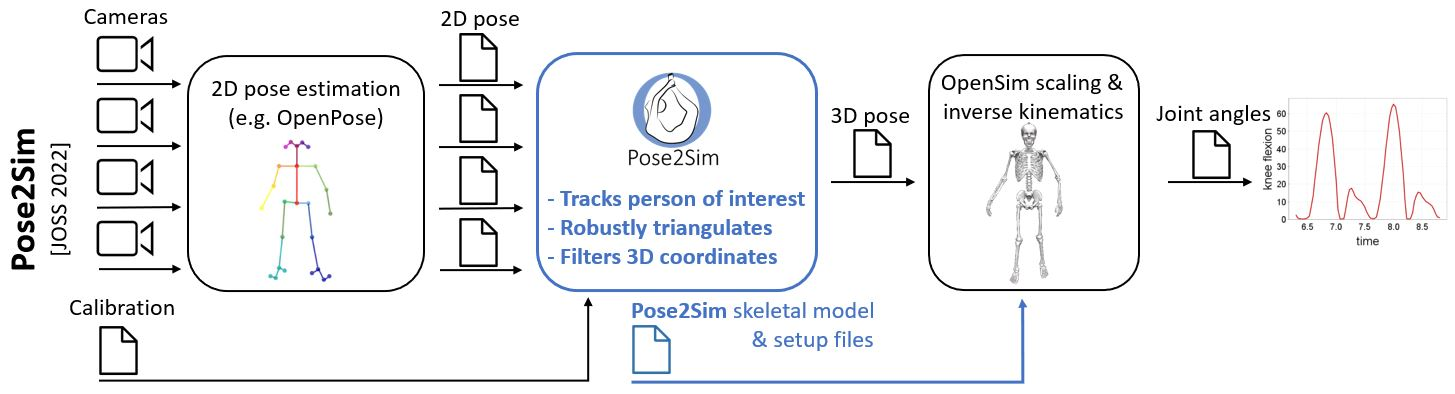
\includegraphics[width=\linewidth]{"../Intro/Figures/Fig_VisAbstract1.JPG"}
            \caption{Visual abstract for the Pose2Sim workflow \cite{Pagnon2022b}.}
            \label{fig_visabstract1_1}
	\end{subfigure}
	\vskip 1cm
	\begin{subfigure}[b]{1\textwidth}
            \centering
            \def\svgwidth{1\columnwidth}
            \fontsize{10pt}{10pt}\selectfont
            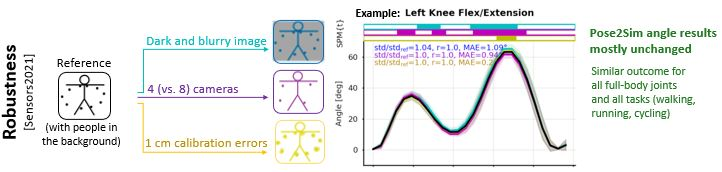
\includegraphics[width=\linewidth]{"../Intro/Figures/Fig_VisAbstract2.JPG"}
            \caption{Visual abstract for Pose2Sim robustness assessment \cite{Pagnon2021}.}
            \label{fig_visabstract2_1}
	\end{subfigure}
	\vskip 1cm
      \begin{subfigure}[b]{1\textwidth}
            \centering
            \def\svgwidth{1\columnwidth}
            \fontsize{10pt}{10pt}\selectfont
            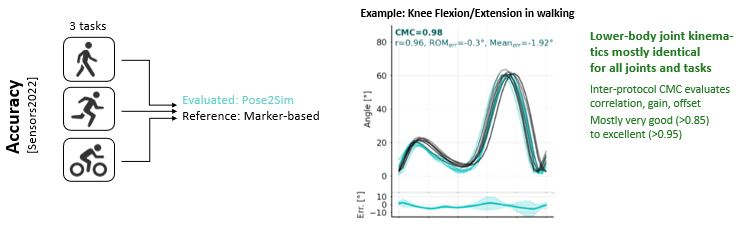
\includegraphics[width=\linewidth]{"../Intro/Figures/Fig_VisAbstract3.JPG"}
            \caption{Visual abstract for Pose2Sim accuracy assessment \cite{Pagnon2022a}.}
            \label{fig_visabstract3_1}
	\end{subfigure}
      \vskip 1cm
	\begin{subfigure}[b]{1\textwidth}
            \centering
            \def\svgwidth{1\columnwidth}
            \fontsize{10pt}{10pt}\selectfont
            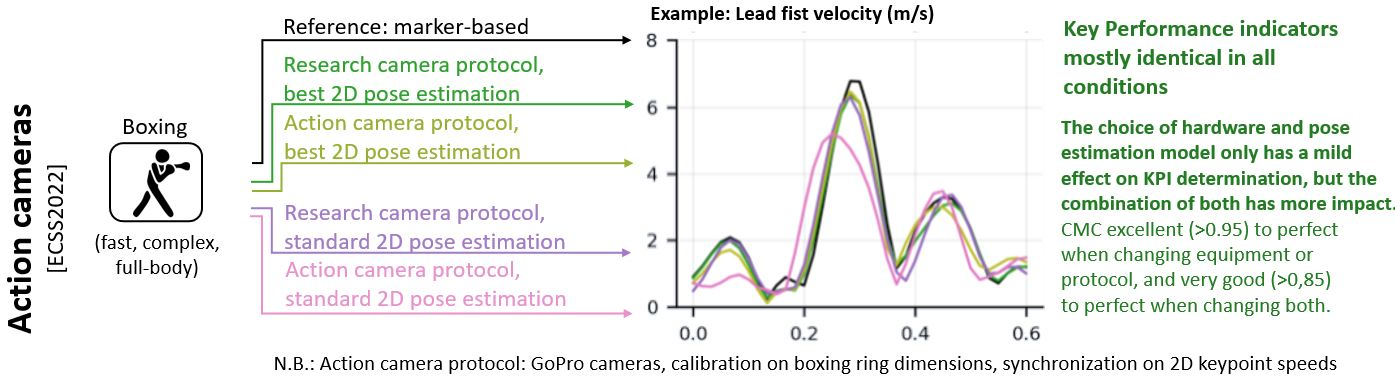
\includegraphics[width=\linewidth]{"../Intro/Figures/Fig_VisAbstract4.JPG"}
            \caption{Visual abstract for the assessment of KPIs in boxing with Pose2Sim \cite{Pagnon2022c}.}
            \label{fig_visabstract4_1}
	\end{subfigure}
	\caption{Visual abstracts for the 4 papers published during this doctoral thesis.}
	\label{fig_visabstract}
\end{figure}


